\section{Fourier Transforms} \label{sec:fouriertransforms}

\subsection{Eigenfunctions and $H(s)$}

An \emph{eigenfunction} $x(t) = e^{j\omega t}$ is a function such that
$S\{x(t)\} = Ax(t)$ for LTI $S$. A property of functions of the form
$e^{j\omega t}$ is that convolution with $h(t)$ yields
\begin{equation}
    x(t) * h(t) = e^{j\omega t} \int_{-\infty}^{\infty} h(\tau) e^{-j\omega \tau} d\tau.
\end{equation}
This is also written as
\begin{equation}
    x(t) * h(t) = e^{j\omega t} \left( |H(j\omega)|e^{j \angle H(j\omega)} \right)
\end{equation}
$H$ is known as the transfer function as has the property that
$Y(S) = H(s)X(s)$, where $Y(s)$ and $X(s)$ are the Laplace transforms
of $y(t)$ and $x(t)$.

\section{Fourier Transform}
Throughout this class we will sometimes see the expression $X(j\omega)$
or $X(e^{j\omega})$.
Note that these are defined as
\begin{equation}
    X(j\omega) = \int_{-\infty}^{\infty} x(t) e^{-j\omega t} dt
\end{equation}
for CT and
\begin{equation}
    X(e^{j\omega}) = \sum_{n=-\infty}^{\infty} x[n] e^{-j\omega n}
\end{equation}
for DT. This transformation is known as the \emph{Fourier Transform}
and works for well-behaved signals.
A signal $x(t)$ is well-behaved iff
\begin{itemize}
    \item $x(t)$ is absolutely integrable over its domain.
    \item $x(t)$ has finite maximum and minimum.
    \item $x(t)$ has finite discontinuities.
\end{itemize}
The original signal can be recovered with
\begin{equation}
    x(t) = \frac{1}{2\pi} \int_{-\infty}^{\infty} X(j\omega) e^{j\omega t} d\omega
\end{equation}
in CT and
\begin{equation}
    x[n] = \frac{1}{2\pi} \int_{-\pi}^{\pi} X(e^{j\omega}) e^{j\omega n} d\omega
\end{equation}
in DT.

If the Fourier series of
\begin{equation}
    x(t) = \sum_{k=-\infty}^{\infty} a_k e^{jk\omega_0 t}
\end{equation}
then the Fourier transform is
\begin{equation}
    X(j\omega) = \sum_{k=-\infty}^{\infty} 2\pi a_k \delta(\omega - k\omega_0).
\end{equation}

This property quickly tells us that the Fourier transform
of $e^{jk\omega_0 t}$ is $2\pi \delta(\omega-k\omega_0)$.
From this the Fourier transforms of sinusoidals quickly follow.

Another important periodic signal is the impulse train,
\begin{equation}
    \sum_{k=-\infty}^{\infty} \delta(t - kT).
\end{equation}
The Fourier series coefficients for
the impulse train are simply $a_k = \frac{1}{T}$,
so the Fourier transform is
$X(j\omega) = \frac{2\pi}{T} \sum_{k=-\infty}^{\infty} \delta(\omega - \frac{2\pi k}{T})$

Note that as $T$ increases, the impulse train gets wider
and wider while its Fourier transform gets narrower and
narrower. This is because, as we will see often, time and
frequency are inversely related. In general, we will find
that
\begin{equation}
    x(at) \leftrightarrow \frac{1}{|a|}X(\frac{j\omega}{a}).
\end{equation}

If $x(t)$ is real, then $|X(j\omega)|$ is even and
$\angle X(j\omega)$ is odd. Moreover, if $x(t)$ is real
and even, then $X(j\omega)$ must be purely real and even,
and if $x(t)$ is real and odd, $X(j\omega)$ is purely
imaginary and odd.

Arguably the most important property we will see is duality.
As an example, a sinc function in time is a rectangular pulse
in frequency, while a rectangular pulse in time is a sinc
function in frequency. Formally,
\begin{equation}
    F\left\{ X(t) \right\} = 2\pi x(-\omega).
\end{equation}

\subsection{Duality}

The Fourier transform displays an interesting symmetry known as duality. 
Figure \ref{fig:duality} shows this graphically. 
\begin{figure}
    \begin{center}
        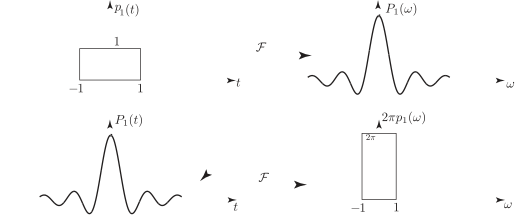
\includegraphics{images/duality.png}
    \end{center}
    \caption{Duality of the Fourier Transform}
    \label{fig:duality}
\end{figure}
Mathematically, if 
\begin{align}
    x(t) \overset{F}{\leftrightarrow} X(j\omega)
\end{align}
then 
\begin{align}
    X(t) \overset{F}{\leftrightarrow} 2\pi x(-\omega).
\end{align}
It doesn't \emph{quite} give you the original function, 
but up to scaling and a reversal you get the original back. 

Some interesting properties derive from duality. Notable ones are:

\begin{itemize}
    \item Differentiation in frequency: If $x(t) \overset{F}{\leftrightarrow} X(j\omega)$, 
    then 
    \begin{equation}
        tx(t)  \overset{F}{\leftrightarrow} j\frac{dX(j\omega)}{d\omega}.
    \end{equation}
    This is the dual property of differentiation in time, 
    \begin{equation}
        \frac{dx(t)}{dt} \overset{F}{\leftrightarrow} j\omega X(j\omega).
    \end{equation}
    \item Frequency shifting: this is the dual of shifting in time. 
    \begin{equation}
        x(t)e^{j\omega_0 t} \overset{F}{\leftrightarrow} X(j(\omega-\omega_0)).
    \end{equation}
    \item Parseval's relation: 
    \begin{align}
        E &= \int_{-\infty}^{\infty} |x(t)|^2 dt \\
        &= \frac{1}{2\pi} \int_{-\infty}^{\infty} |X(j\omega)|^2 d\omega
    \end{align}
\end{itemize}

\subsection{Fourier Transform Properties}

Table \ref{tab:fourier_transform_properties} tabulates
useful properties of Fourier transforms.

\begin{table}[ht]
    \centering
    \caption{Properties of Fourier Transforms}
    \label{tab:fourier_transform_properties}
    \begin{tabular}{llll}
        \toprule
        \textbf{Property}  & \textbf{Time Domain}                &                                          & \textbf{Frequency Domain}                                     \\
        \midrule
        Linearity          & $A x_1(t) + B x_2(t)$               & $\overset{\mathcal{F}}{\leftrightarrow}$ & $A X_1(j\omega) + B X_2(j\omega)$                             \\[1mm]
        Time Shifting      & $x(t - t_0)$                        & $\overset{\mathcal{F}}{\leftrightarrow}$ & $X(j\omega)e^{-j\omega t_0}$                                  \\[1mm]
        Frequency Shifting & $x(t)e^{j\omega_0 t}$               & $\overset{\mathcal{F}}{\leftrightarrow}$ & $X(j(\omega - \omega_0))$                                     \\[1mm]
        Time Scaling       & $x(at)$, $a > 0$                    & $\overset{\mathcal{F}}{\leftrightarrow}$ & $\frac{1}{|a|}X\left(\frac{j\omega}{a}\right)$                \\[1mm]
        Time Reversal      & $x(-t)$                             & $\overset{\mathcal{F}}{\leftrightarrow}$ & $X(-j\omega)$                                                 \\[1mm]
        Conjugation        & $x^*(t)$                            & $\overset{\mathcal{F}}{\leftrightarrow}$ & $X^*(-j\omega)$                                               \\[1mm]
        Differentiation    & $\frac{d^n}{dt^n}x(t)$              & $\overset{\mathcal{F}}{\leftrightarrow}$ & $(j\omega)^n X(j\omega)$                                      \\[1mm]
        Integration        & $\int_{-\infty}^t x(\tau) d\tau$    & $\overset{\mathcal{F}}{\leftrightarrow}$ & $\frac{X(j\omega)}{j\omega} + \pi X(0)\delta(\omega)$         \\[1mm]
        Convolution        & $(x_1 * x_2)(t)$                    & $\overset{\mathcal{F}}{\leftrightarrow}$ & $X_1(j\omega) X_2(j\omega)$                                   \\[1mm]
        Multiplication     & $x_1(t)x_2(t)$                      & $\overset{\mathcal{F}}{\leftrightarrow}$ & $\frac{1}{2\pi}(X_1 * X_2)(j\omega)$                          \\[1mm]
        Parseval's Theorem & $\int_{-\infty}^\infty |x(t)|^2 dt$ & $\overset{\mathcal{F}}{\leftrightarrow}$ & $\frac{1}{2\pi} \int_{-\infty}^\infty |X(j\omega)|^2 d\omega$ \\
        \bottomrule
    \end{tabular}
\end{table}

Table \ref{tab:ctfourier_transforms} tabulates the
Fourier transform of common continuous time functions.

\begin{table}[ht]
    \centering
    \caption{CT Fourier Transforms}
    \label{tab:ctfourier_transforms}
    \begin{tabular}{ll}
        \toprule
        \textbf{Time Domain Function} & \textbf{Fourier Transform}                                                    \\
        \midrule
        $\delta(t)$                   & $1$                                                                           \\[1mm]
        $1$                           & $2\pi\,\delta(\omega)$                                                        \\[1mm]
        $u(t)$                        & $\pi\,\delta(\omega) + \frac{1}{j\omega}$                                     \\[1mm]
        $e^{-at}u(t),\quad \Re(a)>0$  & $\dfrac{1}{a+j\omega}$                                                        \\[1mm]
        $\cos(\omega_0 t)$            & $\pi\Bigl[\delta(\omega-\omega_0) + \delta(\omega+\omega_0)\Bigr]$            \\[1mm]
        $\sin(\omega_0 t)$            & $\dfrac{\pi}{j}\Bigl[\delta(\omega-\omega_0) - \delta(\omega+\omega_0)\Bigr]$ \\[1mm]
        $\mathrm{rect}(t/T)$          & $T\,\mathrm{sinc}\Bigl(\dfrac{\omega T}{2}\Bigr)$                             \\[1mm]
        $e^{-t^2}$                    & $\sqrt{\pi}\,e^{-\omega^2/4}$                                                 \\
        \bottomrule
    \end{tabular}
\end{table}

Table \ref{tab:dtfourier_transforms} tabulates the
Fourier transform of common discrete time functions.

\begin{table}[ht]
    \centering
    \caption{DT Fourier Transforms}
    \label{tab:dtfourier_transforms}
    \begin{tabular}{ll}
        \toprule
        \textbf{Time Domain Function}          & \textbf{Fourier Transform}                                                                                             \\
        \midrule
        $\delta[n]$                            & $1$                                                                                                                    \\[1mm]
        $1$                                    & $2\pi\,\sum_{k=-\infty}^{\infty}\delta(\omega-2\pi k)$                                                                 \\[1mm]
        $a^n u[n],\quad |a|<1$                 & $\dfrac{1}{1-ae^{-j\omega}}$                                                                                           \\[1mm]
        $\cos(\omega_0 n)$                     & $\pi\,\sum_{k=-\infty}^{\infty}\Bigl[\delta(\omega-\omega_0-2\pi k) + \delta(\omega+\omega_0-2\pi k)\Bigr]$            \\[1mm]
        $\sin(\omega_0 n)$                     & $\dfrac{\pi}{j}\,\sum_{k=-\infty}^{\infty}\Bigl[\delta(\omega-\omega_0-2\pi k) - \delta(\omega+\omega_0-2\pi k)\Bigr]$ \\[1mm]
        $\mathrm{rect}\Bigl(\frac{n}{N}\Bigr)$ & $\dfrac{\sin\Bigl(\frac{\omega N}{2}\Bigr)}{\sin\Bigl(\frac{\omega}{2}\Bigr)}\,e^{-j\omega\frac{N-1}{2}}$              \\
        \bottomrule
    \end{tabular}
\end{table}

The most important part of this entire course is the \emph{convolution property}, which states that 
for an LTI system with impulse response $h(t)$, if 
\begin{equation}
    y(t) = x(t) * h(t),
\end{equation}
then
\begin{equation}
    Y(j\omega) = X(j\omega)H(j\omega).
\end{equation}
Essentially, convolution in the time domain is equivalent to multiplication in the frequency domain. 